\documentclass[11pt]{article}

% ---------- packages ----------
\usepackage[a4paper,margin=2.2cm]{geometry}
\usepackage{fontspec}
\setmainfont{Latin Modern Roman}
\usepackage{titlesec}
\usepackage{fancyhdr}
\usepackage{booktabs}
\usepackage{longtable}
\usepackage{array}
\usepackage{listings}
\usepackage{xcolor}
\usepackage{enumitem}
\usepackage{tikz}
\usetikzlibrary{arrows.meta,positioning,fit,backgrounds}
\usepackage{pgfplots}
\pgfplotsset{compat=1.18}
\usepackage{hyperref}
\usepackage{caption}
\usepackage{amsmath}

\hypersetup{
  colorlinks=true,
  linkcolor=violet!70!black,
  citecolor=violet!70!black,
  urlcolor=blue!60!black,
  pdftitle={CS6530 Assignment 1 Report},
  pdfauthor={CS6530 Student}
}

% ---------- fill these in ----------
\newcommand{\StudentName}{\textbf{[YOUR NAME]}}
\newcommand{\RollNumber}{\textbf{[ROLL NUMBER]}}
\newcommand{\SubmissionDate}{August 21, 2026}

% ---------- colors ----------
\definecolor{codebg}{HTML}{F4F4F4}
\definecolor{codeframe}{HTML}{CCCCCC}
\definecolor{passgreen}{HTML}{1E7B3C}
\definecolor{accentamber}{HTML}{9C5F29}
\definecolor{accentteal}{HTML}{2A6F67}

\lstdefinestyle{console}{
  backgroundcolor=\color{codebg},
  basicstyle=\ttfamily\scriptsize,
  breaklines=true,
  frame=single,
  rulecolor=\color{codeframe},
  framesep=6pt,
  xleftmargin=4pt,
  xrightmargin=4pt,
  columns=fullflexible,
  keepspaces=true
}
\lstdefinestyle{cpp}{
  language=C++,
  backgroundcolor=\color{codebg},
  basicstyle=\ttfamily\scriptsize,
  keywordstyle=\color{blue!60!black}\bfseries,
  commentstyle=\color{gray},
  stringstyle=\color{orange!70!black},
  breaklines=true,
  frame=single,
  rulecolor=\color{codeframe},
  framesep=6pt,
  showstringspaces=false
}

\titleformat{\section}{\Large\bfseries\color{accentteal}}{\thesection}{0.6em}{}
\titleformat{\subsection}{\large\bfseries}{\thesubsection}{0.6em}{}

\pagestyle{fancy}
\fancyhf{}
\fancyhead[L]{\small CS6530 -- Applied Cryptography, Assignment 1}
\fancyhead[R]{\small \StudentName}
\fancyfoot[C]{\thepage}
\renewcommand{\headrulewidth}{0.4pt}

% ---------- pass/fail macro ----------
\newcommand{\PASS}{\textcolor{passgreen}{\textbf{PASS}}}

\begin{document}

% ==================== TITLE PAGE ====================
\begin{titlepage}
\centering
\vspace*{1.5cm}
{\Large IIT Madras --- CSE Department}\\[0.3cm]
{\large CS6530 -- Applied Cryptography, Jul--Nov 2026}\\[1.5cm]

{\huge\bfseries Assignment 1 Report}\\[0.6cm]
{\Large Secure Data Protection using AES-GCM and ChaCha20-Poly1305}\\[2cm]

\begin{tabular}{rl}
\textbf{Name:} & \StudentName \\
\textbf{Roll Number:} & \RollNumber \\
\textbf{Submission Date:} & \SubmissionDate \\
\end{tabular}

\vfill
{\small A secure data protection subsystem for generic chunked/packetized application
records, using AES-128-GCM and ChaCha20-Poly1305 authenticated encryption, implemented
in C++17 over OpenSSL's EVP API.}
\end{titlepage}

\tableofcontents
\newpage

% ==================== 1. INTRODUCTION ====================
\section{Introduction}

This report documents the design, implementation, and validation of a secure data
protection subsystem that exchanges application records between a \texttt{Sender} and
a \texttt{Receiver} using Authenticated Encryption with Associated Data (AEAD). The
subsystem supports two interchangeable AEAD configurations -- \textbf{AES-128-GCM} and
\textbf{ChaCha20-Poly1305} -- both accessed through OpenSSL's EVP API, consistent with
the assignment's emphasis on secure integration rather than primitive implementation.

The sender and receiver are assumed to already share a secret key (read from a key
file at start-up); secure key establishment is explicitly out of scope. Network
communication is likewise not required: the two roles exchange protected records
through a shared file, \texttt{tm.bin}, which stands in for a transport channel.

All source code referenced in this report is included in the submission under
\texttt{src/}. Build and run instructions are in the project \texttt{README.md}.

% ==================== 2. DESIGN SUMMARY ====================
\section{Design Summary}

\subsection{Architecture}

The subsystem is organized into five classes, each responsible for exactly one
concern:

\begin{center}
\begin{tabular}{@{}p{2.6cm}p{6.4cm}p{5.5cm}@{}}
\toprule
\textbf{Class} & \textbf{Responsibility} & \textbf{Location} \\
\midrule
\texttt{Record} & The application record: sequence id, timestamp, payload. & \texttt{record.h} \\
\texttt{Serializer} & \texttt{Record} $\leftrightarrow$ fixed-width byte encoding. & \texttt{serializer.\{h,cpp\}} \\
\texttt{Crypt} & AEAD engine: nonce generation, encrypt/decrypt, wire-format framing, for both algorithms. & \texttt{crypt.\{h,cpp\}} \\
\texttt{Sender} & Build record $\to$ serialize $\to$ encrypt $\to$ write channel. & \texttt{sender.\{h,cpp\}} \\
\texttt{Receiver} & Read channel $\to$ decrypt $\to$ verify $\to$ replay-check $\to$ deserialize. & \texttt{receiver.\{h,cpp\}} \\
\bottomrule
\end{tabular}
\end{center}

\begin{figure}[h!]
\centering
\resizebox{\textwidth}{!}{%
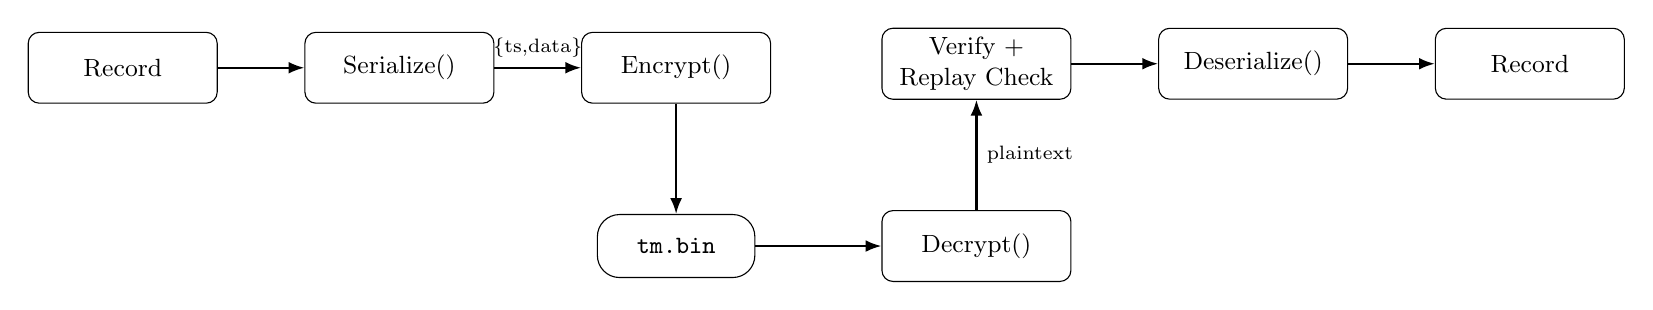
\begin{tikzpicture}[
  box/.style={draw, rounded corners, minimum width=2.4cm, minimum height=0.9cm, align=center, font=\small},
  file/.style={draw, rounded corners=8pt, minimum width=2cm, minimum height=0.8cm, align=center, font=\small\ttfamily},
  lbl/.style={font=\scriptsize, align=center},
  arr/.style={-{Latex[length=2mm]}, thick}
]
\node[box] (rec1) {Record};
\node[box, right=1.1cm of rec1] (ser) {Serialize()};
\node[box, right=1.1cm of ser] (enc) {Encrypt()};
\node[file, below=1.4cm of enc] (tm) {tm.bin};
\node[box, right=1.1cm of tm, xshift=0.5cm] (dec) {Decrypt()};
\node[box, above=1.4cm of dec] (verify) {Verify + \\ Replay Check};
\node[box, right=1.1cm of verify] (des) {Deserialize()};
\node[box, right=1.1cm of des] (rec2) {Record};

\draw[arr] (rec1) -- (ser);
\draw[arr] (ser) -- node[lbl,above]{\{ts,data\}} (enc);
\draw[arr] (enc.south) -- (tm.north);
\draw[arr] (tm.east) -- (dec.west);
\draw[arr] (dec.north) -- node[lbl,right]{plaintext} (verify.south);
\draw[arr] (verify) -- (des);
\draw[arr] (des) -- (rec2);
\end{tikzpicture}%
}
\caption{End-to-end record pipeline. \texttt{tm.bin} stores AAD (4B), nonce
(12B), ciphertext, and tag (16B) concatenated.}
\end{figure}

\subsection{Wire Format}

Each protected record written to \texttt{tm.bin} is a single concatenation of four
fixed-position fields:
\[
\texttt{secureStream} = \underbrace{\texttt{AAD}}_{4\text{ B}} \,\|\, \underbrace{\texttt{nonce}}_{12\text{ B}} \,\|\, \texttt{ciphertext} \,\|\, \underbrace{\texttt{tag}}_{16\text{ B}}
\]
Because every field except the ciphertext has a length fixed by the algorithm choice,
the receiver can slice the blob back apart by fixed offsets without a length-prefixed
or self-describing envelope.

\subsection{Nonce Management (FR-5 / SR-3)}

A fresh 96-bit nonce is generated via OpenSSL's \texttt{RAND\_bytes} (a CSPRNG) for
\emph{every} call to \texttt{Crypt::Encrypt}; no nonce is ever cached, derived from a
counter, or reused. This is the standard nonce strategy for both GCM and
ChaCha20-Poly1305, and needs no persisted state across sender restarts -- the
trade-off is a birthday-bound collision risk that only becomes material after roughly
$2^{32}$ messages under one key, far beyond this subsystem's demonstrated volume (see
TR-7, Section~\ref{sec:tr7}).

\subsection{Associated Data Selection (FR-4 / SR-4)}

The record's 4-byte sequence id is authenticated as AAD. It remains visible in
plaintext on the wire (sequence ids are not secret) but cannot be detached from its
ciphertext, or swapped for a different record's id, without invalidating the
authentication tag. This binding is what makes replay detection possible: the receiver
only trusts a record's id after the tag has verified.

\subsection{Replay Handling Strategy (FR-8 / SR-5)}

The \texttt{Receiver} maintains an in-memory set, \texttt{seenRecIds}, of every record
id it has accepted in the current session. After a record decrypts and its
authentication tag verifies, its id (recovered from the now-trusted AAD) is checked
against this set; a repeat is rejected before \texttt{Receive()} ever returns data to
the caller. This strategy accepts records in any order (not just strictly increasing
ids) and detects a genuine replay unambiguously. Its main limitation -- discussed
further in Section~\ref{sec:discussion} -- is that the set grows without bound for the
life of the session, which a production system would instead bound with a sliding
window (as TLS and IPsec do).

\subsection{Authentication Failure Handling (FR-7 / SR-6)}

OpenSSL's decrypt API only confirms authenticity at \texttt{EVP\_DecryptFinal\_ex},
which returns $\leq 0$ on a tag mismatch; \texttt{EVP\_DecryptUpdate} itself will
produce plaintext-shaped bytes even for a corrupted ciphertext. \texttt{Crypt::Decrypt}
treats the final-step return value as the single point of truth and \emph{throws} on
failure rather than returning a status flag, so a failure can only be silently ignored
by an explicit, conscious \texttt{catch} -- which is exactly the fail-closed behaviour
\texttt{Receiver::ConstructRecord} implements: any exception during decryption,
verification, or replay checking results in \texttt{Receive()} returning an empty
string, with nothing recovered ever exposed to the caller.

\subsection{Key Management (Out of Scope)}

Per the assignment's stated assumptions, the sender and receiver already share a
secret key; this subsystem reads that key from a binary file
(\texttt{keys/aeskey.bin}, 16 bytes for AES-128-GCM; \texttt{keys/ccpkey.bin}, 32 bytes
for ChaCha20-Poly1305). No key exchange, rotation, or derivation is implemented, in
line with the assignment's Section~3.2 scope exclusions.

% ==================== 3. TESTING METHODOLOGY ====================
\section{Testing Methodology}

The assignment specifies three logical entities: a \textbf{Sender} that generates
valid protected records, a \textbf{Malicious Actor} that generates or modifies
protected records to simulate invalid conditions, and a \textbf{Receiver} that
validates and processes received records. All three are realized as logical
components within a single test program, \texttt{src/test\_suite.cpp}, rather than as
separate communicating processes -- an option the assignment explicitly permits
(\emph{``network communication is optional \dots\ provided that all Functional
Requirements and Testing Requirements are satisfied''}).

The malicious actor is implemented as a function, \texttt{CorruptByteAt(offset)}, that
opens \texttt{tm.bin} after a legitimate \texttt{Send()} and flips a single byte via
XOR at a computed offset -- inside the ciphertext, the tag, or the AAD depending on the
test. This achieves the same adversary model as a network-level attacker who can
modify bytes in transit, without the added complexity of standing up sockets or
processes.

Every Testing Requirement below (TR-1 through TR-6) is executed once for AES-128-GCM
and once for ChaCha20-Poly1305, using independent 16-byte and 32-byte keys
respectively, as required by the assignment.

% ==================== 4. TESTING RESULTS ====================
\section{Testing Results}

\subsection{TR-1 -- Positive Baseline Test}

\begin{description}[leftmargin=2.2cm,style=nextline]
\item[Objective] Demonstrate successful protection, transmission, verification, and
recovery of valid application records.
\item[Procedure] Construct a \texttt{Sender} and \texttt{Receiver} sharing the same
key and AEAD configuration. Call \texttt{Sender::Send(msg)}, then
\texttt{Receiver::Receive()}, and compare the recovered string to \texttt{msg}.
\item[Test Input] \texttt{"TR-1 baseline message for AES-128-GCM"} / \texttt{"...for
ChaCha20-Poly1305"}
\item[Expected Behaviour] The recovered string exactly equals the original input.
\item[Observed Behaviour] Recovered string matched the input for both configurations.
\item[Outcome] \PASS\ (AES-128-GCM), \PASS\ (ChaCha20-Poly1305)
\end{description}
\begin{lstlisting}[style=console]
[PASS] TR-1 - Positive baseline (AES-128-GCM)
[PASS] TR-1 - Positive baseline (ChaCha20-Poly1305)
\end{lstlisting}

\subsection{TR-2 -- Ciphertext Integrity Test}

\begin{description}[leftmargin=2.2cm,style=nextline]
\item[Objective] Demonstrate that modification of the protected record's ciphertext
causes authentication failure and rejection by the receiver.
\item[Procedure] Send a valid record, then have the malicious actor flip one byte at
offset~16 of \texttt{tm.bin} -- the first byte of the ciphertext (immediately after the
4-byte AAD and 12-byte nonce) -- before calling \texttt{Receive()}.
\item[Test Input] \texttt{"TR-2 ciphertext tamper test"}, tampered at byte offset 16.
\item[Expected Behaviour] \texttt{Receive()} returns an empty string; no plaintext is
released.
\item[Observed Behaviour] \texttt{Receive()} returned \texttt{""} for both
configurations (verified via \texttt{received.empty()}).
\item[Outcome] \PASS\ (AES-128-GCM), \PASS\ (ChaCha20-Poly1305)
\end{description}
\begin{lstlisting}[style=console]
[PASS] TR-2 - Ciphertext integrity (AES-128-GCM)
[PASS] TR-2 - Ciphertext integrity (ChaCha20-Poly1305)
\end{lstlisting}

\subsection{TR-3 -- Authentication Tag Test}

\begin{description}[leftmargin=2.2cm,style=nextline]
\item[Objective] Demonstrate that modification of the authentication tag causes
verification failure and rejection.
\item[Procedure] Send a valid record, then flip the final byte of \texttt{tm.bin} --
which always falls within the trailing 16-byte tag regardless of payload length --
before calling \texttt{Receive()}.
\item[Test Input] \texttt{"TR-3 tag tamper test"}, tampered at the last byte.
\item[Expected Behaviour] \texttt{Receive()} returns an empty string.
\item[Observed Behaviour] \texttt{Receive()} returned \texttt{""} for both
configurations.
\item[Outcome] \PASS\ (AES-128-GCM), \PASS\ (ChaCha20-Poly1305)
\end{description}
\begin{lstlisting}[style=console]
[PASS] TR-3 - Authentication tag (AES-128-GCM)
[PASS] TR-3 - Authentication tag (ChaCha20-Poly1305)
\end{lstlisting}

\subsection{TR-4 -- Associated Data (AAD) Test}

\begin{description}[leftmargin=2.2cm,style=nextline]
\item[Objective] Demonstrate that modification of the Associated Data causes
verification failure and rejection.
\item[Procedure] Send a valid record, then flip byte offset~0 of \texttt{tm.bin} --
inside the 4-byte AAD (record id) -- before calling \texttt{Receive()}.
\item[Test Input] \texttt{"TR-4 AAD tamper test"}, tampered at byte offset 0.
\item[Expected Behaviour] \texttt{Receive()} returns an empty string.
\item[Observed Behaviour] \texttt{Receive()} returned \texttt{""} for both
configurations.
\item[Outcome] \PASS\ (AES-128-GCM), \PASS\ (ChaCha20-Poly1305)
\end{description}
\begin{lstlisting}[style=console]
[PASS] TR-4 - AAD integrity (AES-128-GCM)
[PASS] TR-4 - AAD integrity (ChaCha20-Poly1305)
\end{lstlisting}

\subsection{TR-5 -- Replay Test}

\begin{description}[leftmargin=2.2cm,style=nextline]
\item[Objective] Demonstrate that replay of a previously accepted protected record is
detected and rejected.
\item[Procedure] Send one valid record and call \texttt{Receive()} once (expected to
succeed). Without any further \texttt{Send()}, call \texttt{Receive()} again on the
same, unchanged \texttt{tm.bin} -- simulating an attacker resubmitting a captured
record.
\item[Test Input] \texttt{"TR-5 replay test"}, received twice.
\item[Expected Behaviour] The first \texttt{Receive()} returns the original message;
the second returns an empty string.
\item[Observed Behaviour] First call succeeded and matched the input; second call
returned \texttt{""} for both configurations (rejected via the \texttt{seenRecIds}
check in \texttt{Receiver::ConstructRecord}).
\item[Outcome] \PASS\ (AES-128-GCM), \PASS\ (ChaCha20-Poly1305)
\end{description}
\begin{lstlisting}[style=console]
[PASS] TR-5 - Replay handling (AES-128-GCM)
[PASS] TR-5 - Replay handling (ChaCha20-Poly1305)
\end{lstlisting}

\subsection{TR-6 -- Wrong-Key Test}

\begin{description}[leftmargin=2.2cm,style=nextline]
\item[Objective] Demonstrate that use of an incorrect cryptographic key causes
verification failure and rejection.
\item[Procedure] Send a record encrypted under one key; construct the
\texttt{Receiver} with a different key of the same length (16 bytes for AES-128-GCM,
32 for ChaCha20-Poly1305) and call \texttt{Receive()}.
\item[Test Input] \texttt{"TR-6 wrong key test"}, decrypted with a mismatched key.
\item[Expected Behaviour] \texttt{Receive()} returns an empty string.
\item[Observed Behaviour] \texttt{Receive()} returned \texttt{""} for both
configurations.
\item[Outcome] \PASS\ (AES-128-GCM), \PASS\ (ChaCha20-Poly1305)
\end{description}
\begin{lstlisting}[style=console]
[PASS] TR-6 - Wrong-key rejection (AES-128-GCM)
[PASS] TR-6 - Wrong-key rejection (ChaCha20-Poly1305)
\end{lstlisting}

\subsection{TR-7 -- Nonce Management Verification}
\label{sec:tr7}

\begin{description}[leftmargin=2.2cm,style=nextline]
\item[Objective] Demonstrate that the nonce management approach (Section~2.3) prevents
nonce reuse under normal operation, per the assignment's guideline of processing
approximately 10{,}000 records under one key.
\item[Procedure] Using a single \texttt{Sender} instance and a fixed key, send 10{,}000
records in sequence. After each \texttt{Send()}, read the 12-byte nonce field back out
of \texttt{tm.bin} (offset~4, immediately after the AAD) and insert it into a
\texttt{std::set}. A collision would shrink the set below the message count.
\item[Test Input] 10{,}000 sequential records (\texttt{"nonce-test-record-0"} \dots
\texttt{"nonce-test-record-9999"}), one key per algorithm.
\item[Expected Behaviour] The set of observed nonces contains exactly 10{,}000 unique
entries -- zero collisions.
\item[Observed Behaviour] 10{,}000 unique nonces observed for both configurations, with
no duplicate detected at any of the 1{,}000-record progress checkpoints.
\item[Outcome] \PASS\ (AES-128-GCM), \PASS\ (ChaCha20-Poly1305)
\end{description}
\begin{lstlisting}[style=console]
--- TR-7: Nonce Management Verification ---
No reuse detected till 1000th iteration
No reuse detected till 2000th iteration
No reuse detected till 3000th iteration
No reuse detected till 4000th iteration
No reuse detected till 5000th iteration
No reuse detected till 6000th iteration
No reuse detected till 7000th iteration
No reuse detected till 8000th iteration
No reuse detected till 9000th iteration
[PASS] TR-7 - Nonce uniqueness over 10000 records (AES-128-GCM) (10000 unique nonces observed)
No reuse detected till 1000th iteration
...
No reuse detected till 9000th iteration
[PASS] TR-7 - Nonce uniqueness over 10000 records (ChaCha20-Poly1305) (10000 unique nonces observed)
\end{lstlisting}

\subsection*{Correctness Summary}
\begin{center}
\begin{tabular}{lccc}
\toprule
\textbf{Requirement} & \textbf{AES-128-GCM} & \textbf{ChaCha20-Poly1305} & \textbf{Total} \\
\midrule
TR-1 -- Positive baseline & \PASS & \PASS & 2/2 \\
TR-2 -- Ciphertext integrity & \PASS & \PASS & 2/2 \\
TR-3 -- Authentication tag & \PASS & \PASS & 2/2 \\
TR-4 -- AAD integrity & \PASS & \PASS & 2/2 \\
TR-5 -- Replay handling & \PASS & \PASS & 2/2 \\
TR-6 -- Wrong-key rejection & \PASS & \PASS & 2/2 \\
TR-7 -- Nonce uniqueness (10{,}000 msgs) & \PASS & \PASS & 2/2 \\
\midrule
\textbf{Total} & \textbf{7/7} & \textbf{7/7} & \textbf{14/14} \\
\bottomrule
\end{tabular}
\end{center}

% ==================== 5. PERFORMANCE ====================
\section{Performance Analysis (TR-8)}

\subsection*{Objective and Procedure}
Compare AES-128-GCM and ChaCha20-Poly1305 by measuring encrypt/decrypt cost at three
payload sizes -- 64~B, 1~KiB, and 64~KiB -- as required by the assignment. Timing is
taken directly around \texttt{Crypt::Encrypt}/\texttt{Decrypt} (bypassing
\texttt{Sender}/\texttt{Receiver}'s file I/O), since disk I/O time would otherwise
dominate and mask the actual cost difference between the two ciphers; this is a
deliberate scoping decision, not an oversight. Each measurement is averaged over 2{,}000
iterations (500 for 64~KiB, to keep total runtime reasonable), using
\texttt{std::chrono::high\_resolution\_clock}. All measurements were taken on an Intel
Core~i5-12450H (12th Gen), which exposes the \texttt{AES-NI} and \texttt{PCLMULQDQ}
instruction extensions.

\subsection*{Observed Results}
\begin{center}
\begin{tabular}{llrrrr}
\toprule
\textbf{Algorithm} & \textbf{Size} & \textbf{Encrypt ($\mu$s)} & \textbf{Decrypt ($\mu$s)} & \textbf{Enc MB/s} & \textbf{Dec MB/s} \\
\midrule
AES-128-GCM        & 64 B   & 2.27  & 1.21  & 26.95  & 50.57 \\
ChaCha20-Poly1305  & 64 B   & 2.14  & 1.29  & 28.49  & 47.41 \\
AES-128-GCM        & 1 KiB  & 2.82  & 1.36  & 346.08 & 715.91 \\
ChaCha20-Poly1305  & 1 KiB  & 3.38  & 2.00  & 288.98 & 487.11 \\
AES-128-GCM        & 64 KiB & 88.67 & 30.38 & 704.88 & 2057.10 \\
ChaCha20-Poly1305  & 64 KiB & 112.55 & 81.05 & 555.31 & 771.15 \\
\bottomrule
\end{tabular}
\end{center}

\begin{figure}[h!]
\centering
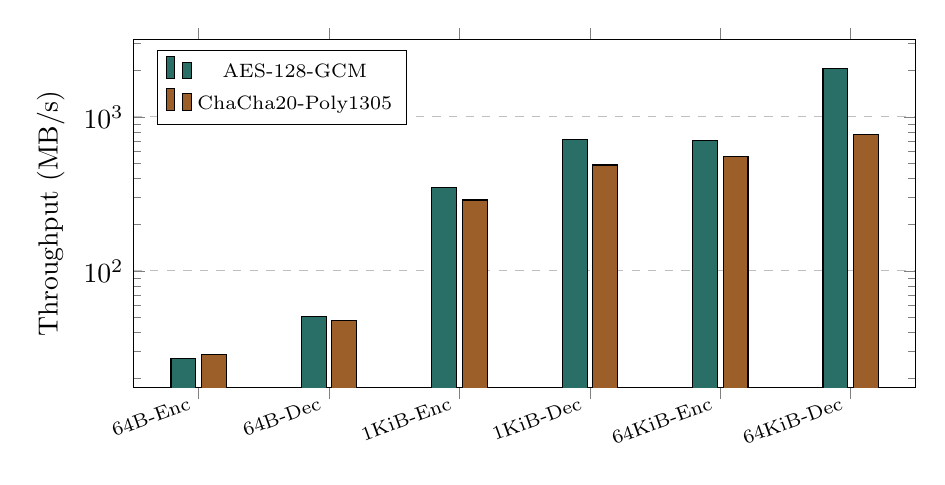
\begin{tikzpicture}
\begin{axis}[
  ybar, bar width=9pt,
  width=0.95\textwidth, height=6cm,
  symbolic x coords={64B-Enc,64B-Dec,1KiB-Enc,1KiB-Dec,64KiB-Enc,64KiB-Dec},
  xtick=data,
  x tick label style={rotate=20,anchor=east,font=\scriptsize},
  ylabel={Throughput (MB/s)},
  ymajorgrids=true, grid style=dashed,
  legend pos=north west, legend style={font=\scriptsize},
  ymode=log, log basis y=10,
]
\addplot[fill=accentteal] coordinates {
  (64B-Enc,26.95) (64B-Dec,50.57)
  (1KiB-Enc,346.08) (1KiB-Dec,715.91)
  (64KiB-Enc,704.88) (64KiB-Dec,2057.10)
};
\addplot[fill=accentamber] coordinates {
  (64B-Enc,28.49) (64B-Dec,47.41)
  (1KiB-Enc,288.98) (1KiB-Dec,487.11)
  (64KiB-Enc,555.31) (64KiB-Dec,771.15)
};
\legend{AES-128-GCM, ChaCha20-Poly1305}
\end{axis}
\end{tikzpicture}
\caption{Throughput by payload size and operation (log scale).}
\end{figure}

\subsection*{Discussion}
At 64~B, the two algorithms are within noise of each other -- fixed per-call overhead
(EVP context setup) dominates at that size rather than the cipher's steady-state
throughput. From 1~KiB onward, AES-128-GCM pulls ahead by roughly 1.2--2$\times$. This is
directly attributable to hardware acceleration: this CPU's \texttt{AES-NI} instruction
computes one AES round per instruction, and \texttt{PCLMULQDQ} similarly accelerates
GCM's GHASH computation, while ChaCha20-Poly1305 has no equivalent hardware fast path
and executes as general-purpose ARX/polynomial arithmetic on the ALU regardless of the
underlying CPU. On hardware \emph{without} AES-NI -- common on low-end ARM cores and
some embedded/IoT targets -- this result would invert, which is precisely why
ChaCha20-Poly1305 is standardized as a TLS~1.3 cipher suite alongside AES-GCM rather
than superseded by it.

% ==================== 6. DISCUSSION ====================
\section{Discussion}
\label{sec:discussion}

\subsection*{Implementation Assumptions}
\begin{itemize}[leftmargin=1.2cm]
\item The sender and receiver share a pre-provisioned key, read from a local file; no
key exchange or rotation is implemented (assignment Section~3.2).
\item \texttt{tm.bin} is treated purely as a byte-transport abstraction; no access
control on the file itself is assumed necessary, since the AEAD tag already defends
against undetected tampering by anyone able to write to it.
\item The replay-protection set (\texttt{seenRecIds}) is unbounded and scoped to a
single \texttt{Receiver} instance's lifetime -- adequate for this assignment's
demonstrated volume (up to 10{,}000 records per TR-7), but a long-running service would
need a bounded sliding window instead (as used by TLS record replay windows and IPsec
ESP anti-replay windows) to avoid unbounded memory growth.
\item TR-8 performance is measured on the \texttt{Crypt} layer directly, bypassing file
I/O, to isolate cryptographic cost from disk latency.
\end{itemize}

\subsection*{Configuration Equivalence (FR-9)}
Both AEAD configurations are exercised through the identical \texttt{Sender}/
\texttt{Receiver}/\texttt{Crypt} interface and pass an identical set of TR-1 through
TR-7 checks; the only externally visible difference is the required key length (16
bytes vs.\ 32 bytes) and, as shown in Section~5, runtime performance.

\subsection*{Limitations}
\begin{itemize}[leftmargin=1.2cm]
\item No key rotation or expiry mechanism.
\item No transport-level authentication of \texttt{tm.bin} itself, beyond what the
AEAD tag already provides for the payload.
\item \texttt{Sender::sendCount} is a single process-wide counter; a multi-sender
deployment sharing one key would additionally need a partitioned nonce/id scheme (a
fixed sender-id prefix plus a local counter, as used by QUIC and IPsec Security
Associations) to keep id/nonce spaces disjoint across senders.
\end{itemize}
None of these are deficiencies relative to the assignment's stated scope -- they are
documented boundaries of what was intentionally left out, consistent with
Section~3.2 of the assignment brief.

% ==================== 7. CONCLUSION ====================
\section{Conclusion}

The implemented subsystem satisfies all stated Functional and Security Requirements:
both AEAD configurations correctly protect and recover application records
(FR-1--FR-3, FR-9), Associated Data and authentication tags are verified before any
plaintext is released (FR-4, FR-6, FR-7, SR-1, SR-2, SR-4, SR-6), nonces are generated
freshly per message with empirically zero collisions across 10{,}000 records per
algorithm (FR-5, SR-3), and replayed records are detected and rejected (FR-8, SR-5).
All 14 correctness checks (TR-1--TR-7, across both configurations) pass, and the
performance comparison (TR-8) shows AES-128-GCM outperforming ChaCha20-Poly1305 by
roughly 1.2--2$\times$ on this AES-NI-equipped machine, consistent with the expected
behaviour of a hardware-accelerated versus software-only AEAD construction.

\end{document}
